\documentclass[tikz,border=2pt]{standalone}
\usepackage{amsmath}
\usepackage{pgfplots}
\pgfplotsset{compat=1.18}

\begin{document}
% Minimising f is the same as maximising -f: the graphs are mirror images, the optimal x is
% the same, and the optimal values are negatives of each other.
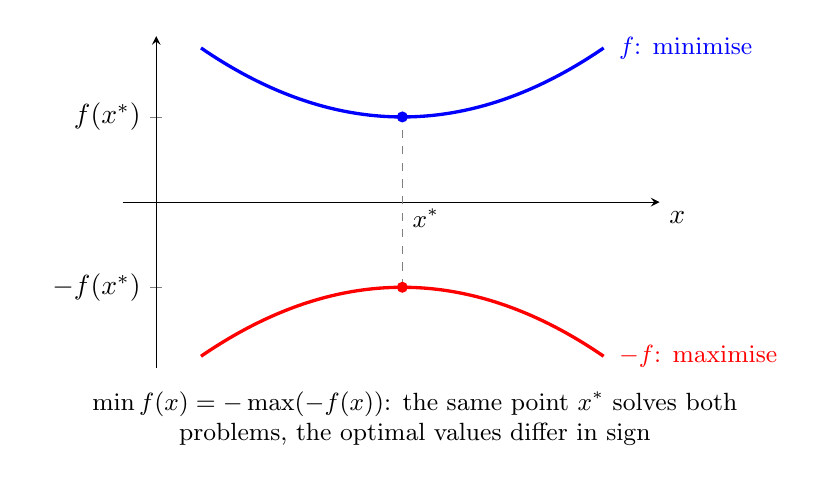
\begin{tikzpicture}
	\begin{axis}[
		axis lines=middle, xmin=-0.3, xmax=4.5, ymin=-3.9, ymax=3.9,
		xtick=\empty, ytick={-2,2}, yticklabels={$-f(x^\ast)$,$f(x^\ast)$},
		xlabel={$x$}, xlabel style={below right},
		samples=80, smooth, width=8.4cm, height=5.8cm, clip=false
		]
		\addplot[blue, very thick, domain=0.4:4] {0.5*(x-2.2)^2+2};
		\addplot[red, very thick, domain=0.4:4] {-0.5*(x-2.2)^2-2};
		\draw[gray, dashed] (axis cs:2.2,-2) -- (axis cs:2.2,2);
		\fill[blue] (axis cs:2.2,2) circle (2pt);
		\fill[red] (axis cs:2.2,-2) circle (2pt);
		\node[anchor=north west, font=\small, inner sep=1.5pt] at (axis cs:2.25,-0.05) {$x^\ast$};
		\node[blue, anchor=west, font=\small] at (axis cs:4.05,3.62) {$f$: minimise};
		\node[red, anchor=west, font=\small] at (axis cs:4.05,-3.62) {$-f$: maximise};
	\end{axis}
	\node[anchor=north, font=\small, align=flush center, text width=9.6cm] at ([yshift=-2pt]current axis.outer south) {$\min f(x)=-\max(-f(x))$: the same point $x^\ast$ solves both problems, the optimal values differ in sign};
\end{tikzpicture}
\end{document}
